\documentclass{article}
\usepackage[a4paper, total={7in, 10in}]{geometry}
\usepackage[utf8]{inputenc}
\usepackage{graphicx}

\graphicspath{ {./images/} }

% New commands
    \newcommand{\vect}[1]{\left[\begin{array}{c}#1\end{array}\right]}
% 

\title{SyArm Positioning}
\author{Samuel Nösslböck}
\date{April 2022}

\begin{document}

\maketitle

\section{Introduction}
    The SyArm is build up from two arms and a tong, represented by three vectors. 
    
    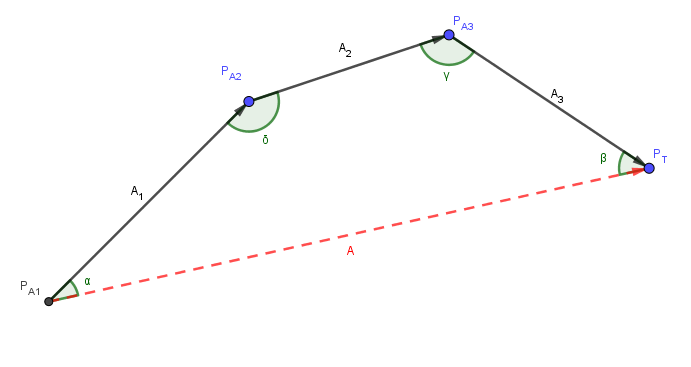
\includegraphics[scale=0.4]{images/Schematic.PNG}
    
    The robot is controlled by a Raspberry PI 3 with a simple systemd service which keeps the main python script alive. 
    
    The main positioning function just receives the three dimensional vector $\vec{A}$ and has to calculate all for the positioning relevant servo angles. 
    
    So the control script knows:
    
    - All lengths $\vec{A}, A_{10}, A_{20}, A_{30}$
    
    - Another property $\delta = \gamma$
    
    An should calculate
    
    - The servo angles $\phi_B, \phi_{A1}, \phi_{A2}, \phi_{T1}$
    
    - The arm vectors $\vec{A_1}, \vec{A_2}, \vec{A_3}$
    
\section{Base Angle $\phi_B$}
    As the unmodified vectors all point along the Y-Axis, the base angle is the only angle that can move all arms towards the target and “create” a X-coordinate.
    
    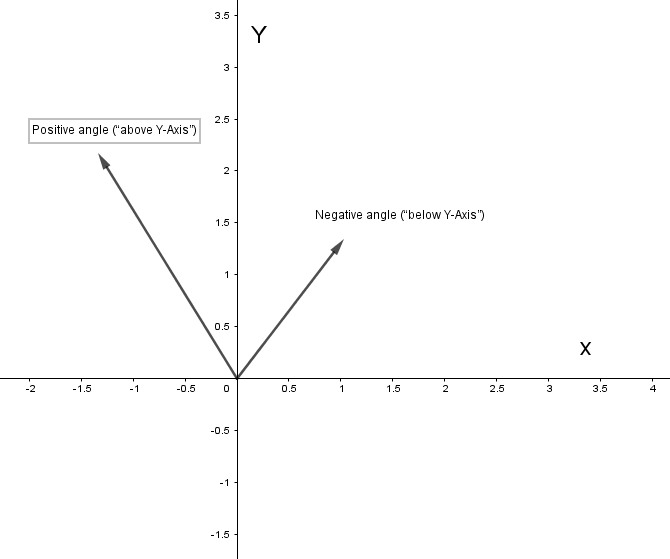
\includegraphics[scale=0.4]{images/ArcSin_Problem.PNG}
    
    Because of this default Y-Axis, the system for a “positive” base angle is rotated by 90 degrees. Which means $\arcsin(y) $ cannot be applied here, the fully defined arc-function for this case is
    
    \begin{equation}
        \phi_B(\vec{A}) =\left\{
        \begin{array}{cc}
            \arcsin(-\hat{x}) & \textit{if}\ \hat{y} > 0 \ \\
            \pi + \arcsin(-\hat{x}) & \textit{otherwise}
        \end{array}\right. \quad
        \hat{x} = \frac{\vec{A}_x}{\sqrt{\vec{A}_x^2 + \vec{A}_y^2}}, \quad
        \hat{y} = \frac{\vec{A}_y}{\sqrt{\vec{A}_x^2 + \vec{A}_y^2}}
    \end{equation}
    
\section{Arm angles}
    To simplify the following equations simpler labels have been assigned to the following labels: 
    
    $a = \vec{A}, \quad b = \vec{A_3}, \quad c = \vec{A_2}, \quad d = \vec{A_1}$ 
    
    As we have all lengths of our polygon, we can extend the lengths $b$ and $d$, to create a triangle.
    
    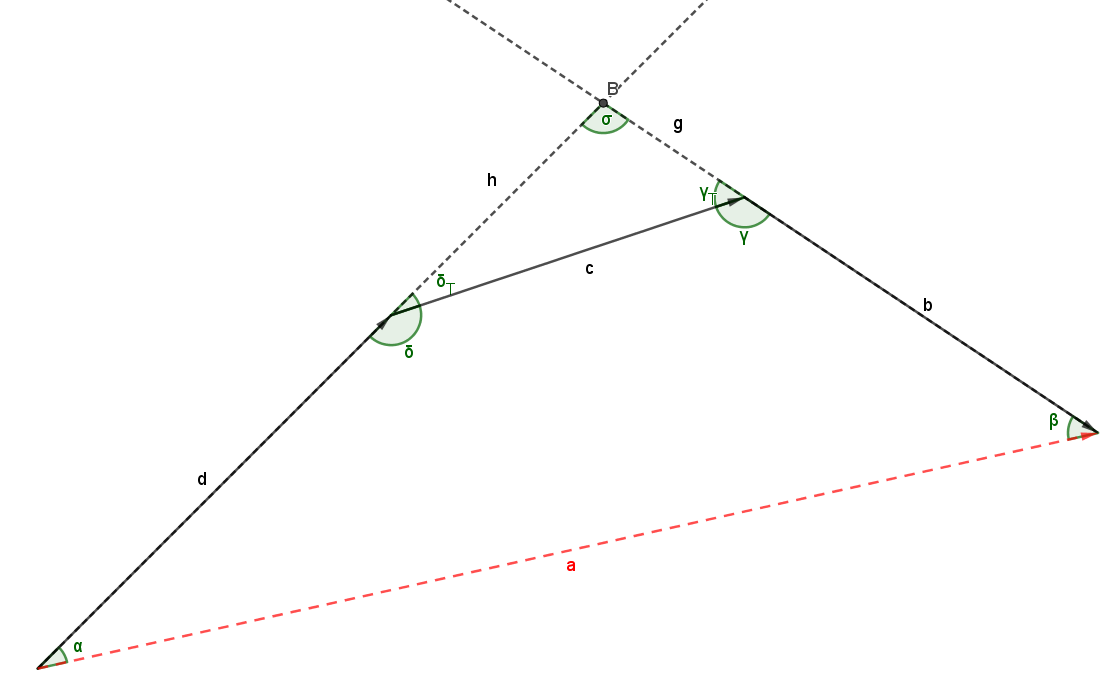
\includegraphics[scale=0.5]{images/polySchematic.PNG}
    
    Considering the property $\delta = \gamma$ the following equations form
        \begin{equation} 360 = \alpha + \beta + \gamma + \delta \newline x\end{equation}
        \begin{equation} 180 = \alpha + \beta + \sigma = \delta_T + \gamma_T + \sigma \end{equation}
        \begin{equation} 180 = \delta + \delta_T = \gamma + \gamma_T \end{equation}
        
        \begin{equation} \delta_T = \gamma_T \quad g = h \end{equation}
    
    As there are now two triangles, one of them being an isosceles one, the law of cosines can be applied
    
        \begin{equation} 
        c^2 = h^2 + g^2 - 2gh\cos(\sigma) = 2g^2 ( 1 - \cos(\sigma) )
        \end{equation}
        \begin{equation} 
        a^2 = (d + g)^2 + (b + g)^2 - 2(d + g)(b + g)\cos(\sigma)
        \end{equation}
    
    Out of equation (6), the cosine of sigma can be calculated with
        \begin{equation} 
        \cos(\sigma) = 1 - \frac{c^2}{2g^2}
        \end{equation}
    
    When this result is inserted into equation (7) we can solve the unknown length g
        \begin{equation} 
        \begin{array}{cc}
                a^2 = (d + g)^2 + (b + g)^2 - 2(d + g)(b + g)(1 - \frac{c^2}{2g^2}) \\
                0 = d^2 + 2dg + g^2 + b^2 + 2bg + g^2 - 2db + \frac{dbc^2}{g^2} - 2dg + \frac{dc^2}{g} - 2gb + \frac{bc^2}{g} - 2g^2 + c^2 \\
                0 = (-a^2 + b^2 + c^2 + d^2 - 2db) + \frac{1}{g}(dc^2 + bc^2) + \frac{1}{g^2}(dbc^2) \\
                0 = g^2 (-a^2 + b^2 + c^2 + d^2 - 2db) + g (dc^2 + bc^2) + dbc^2
        \end{array}
        \end{equation}
    
    For calculation, some helper variables are introduced
        \begin{equation} 
        \begin{array}{cc}
                a_C = -a^2 + b^2 + c^2 + d^2 - 2db\\
                b_C = dc^2 + bc^2\\
                c_C = dbc^2 
        \end{array}
        \end{equation}
        \begin{equation} 
        g_{1,2} = -\frac{b_C}{2a_C} \pm \sqrt{(\frac{b_C}{2a_C})^2 - \frac{c_C}{a_C}}
        \end{equation}
    
    When having the first result for $g$ [$g_1$], equation (8) can be used to calculate $\sigma$, $\gamma$ and $\delta$
        \begin{equation} 
        \begin{array}{cc}
                \sigma = \arccos(1 - \frac{c^2}{2g^2}) \\
                \gamma_T = \frac{180 - \sigma}{2} \\
                \gamma = \delta = 180 - \gamma_T
        \end{array}
        \end{equation}
    
    When now having $\sigma$ and the length of $g$, the law of sines can be applied
        \begin{equation} 
        \frac{a}{\sin(\sigma)} = \frac{d + h}{\sin(\beta)} = \frac{b + g}{\sin(\alpha)}
        \end{equation}
    
    So $\alpha$ and $\beta$ result in 
        \begin{equation}
            \alpha = \arcsin(\frac{\sin(\sigma)(b + g)}{a})
        \end{equation}
        \begin{equation}
            \beta = \arcsin(\frac{\sin(\sigma)(d + h)}{a})
        \end{equation}

\section{Arm vectors}
    The points of each joint and the final position vector can be calculated by using the default vectors
        \begin{equation}
            \vec{A_{10}} = \vec{A_1}(\phi_B = 0, \phi_{A1} = 0) = \vect{0 \\ A_{10} \\ 0}
        \end{equation}
    
        \begin{equation}
            \vec{A_{20}} = \vec{A_2}(\phi_B = 0, \phi_{A1} = 0, \phi_{A2} = 0) = \vect{0 \\ A_{20} \\ 0}
        \end{equation}
    
        \begin{equation}
            \vec{A_{30}} = \vec{A_3}(\phi_B = 0, \phi_{A1} = 0, \phi_{A2} = 0, \phi_{A3} = 0) = \vect{ 0 \\ A_{30} \\ 0}
        \end{equation}
    
    and rotating around the servo axis using rotation matrices. The base rotation is represented by a Z-axis rotation, the joints by a X-axis rotation
    
        \begin{equation}
            \vec{A_1}(\phi_B, \phi_{A1}) = R_Z(\phi_B) \cdot R_X(\phi_{A1}) \cdot \vec{A_{10}}; \quad
            P_{A1} = \vect{0 \\ 0 \\ 0} \quad
            P_{A2}(\phi_B, \phi_{A1}) = P_{A1} + \vec{A_1}(\phi_B, \phi_{A1})
        \end{equation}
        
        \begin{equation}
            \vec{A_2}(\phi_B, \phi_{A1}, \phi_{A2}) = R_Z(\phi_B) \cdot R_X(\phi_{A1}) \cdot R_X(\phi_{A2}) \cdot \vec{A_{20}} \quad
            P_{A3}(\phi_B, \phi_{A1}, \phi_{A2}) = P_{A2} + \vec{A_2}(\phi_B, \phi_{A1}, \phi_{A2})
        \end{equation}
        
        \begin{equation}
            \begin{array}{cc}
                \vec{A_3}(\phi_B, \phi_{A1}, \phi_{A2}, \phi_{A3}) = R_Z(\phi_B) \cdot R_X(\phi_{A1}) \cdot R_X(\phi_{A2}) \cdot R_X(\phi_{A3}) \cdot \vec{A_{30}} \\
                P_{T1}(\phi_B, \phi_{A1}, \phi_{A2}, \phi_{A3}) = P_{A3} + \vec{A_3}(\phi_B, \phi_{A1}, \phi_{A2}, \phi_{A3})
            \end{array}
        \end{equation}
    
    Taking all of these vectors, the position vector $\vec{A}$ can be calculated 
        
        \begin{equation}
            \begin{array}{cc}
                \vec{A}(\phi_B, \phi_{A1}, \phi_{A2}, \phi_{A3}) = \vec{A_1}(\phi_B, \phi_{A1}) + \vec{A_2}(\phi_B, \phi_{A1}, \phi_{A2}) + \vec{A_3}(\phi_B, \phi_{A1}, \phi_{A2}, \phi_{A3}) \\
                
                \vec{A}(\phi_B, \phi_{A1}, \phi_{A2}, \phi_{A3}) = R_Z(\phi_B) \cdot R_X(\phi_{A1}) \cdot \left( \vec{A_{10}}  + R_X(\phi_{A2}) \cdot \left( \vec{A_{20}}  + R_X(\phi_{A3}) \cdot \vec{A_{30}} \right) \right)
            \end{array}
        \end{equation} 
    
    \clearpage
    
\section{Coordinate systems and conversions}
    The control script uses multiple coordinate systems listed here
    \begin{equation}
        \textit{Kath} = \vect{x \\ y \\ z} \qquad \textit{Rot} = \vect{r \\ \phi_Z \\ \phi_X }
    \end{equation}
    
    Kath and Rot both have their advantages and disadvantages, Rot is easier to use for the control system (it always converts to this system), while Kath is easier for human use. The conversion functions are the following
    \begin{equation}
        \textit{Kath}(\textit{Rot}) = R_Z(\phi_Z) \cdot R_X(\phi_X) \cdot \vect{0 \\ r \\ 0}
    \end{equation}
    
    \begin{equation}
        \textit{Rot}(\textit{Kath}) = \vect{|\textit{Kath}| \\ \arctan_F(y, -x) \\ \arctan_F(\sqrt{x^2 + y^2}, z)} \quad
        \arctan_F(x, y) =\left\{
        \begin{array}{cc}
            \arctan(y / x) & \textit{if}\ x > 0 \ \\
            \pi + \arctan(y / x) & \textit{if} \ x < 0 \ \\
            
            \left\{\begin{array}{cc}
                \frac{\pi}{2} & \textit{if}\ y > 0 \ \\
                \frac{-\pi}{2} & \textit{if}\ y < 0 \ \\
                0 & \textit{otherwise}
            \end{array}\right. & \textit{otherwise} 
        \end{array}\right. 
    \end{equation}

\end{document}